\chapter{Maximum Contiguous Subsequence Sum}
\label{ch:mcss}

\begin{preamble}
This chapter reviews the classic problem of finding the contiguous
subsequence of a sequence with the maximal value, 
%
and provides several algorithms for the problem by applying several design techniques including
\href{sec:design::bf}{brute force},
%
\href{sec:design::reduction}{reduction}, and
%
\href{ch:design::dc}{divide and conquer}.
%

\end{preamble}


\section{The Problem}
\label{sec:mcss::problem}

\begin{teachnote}
This lecture needs a bit more structure.  There are quie a few moving
pieces complete the plot below and use it as a guide.  

There are some glitches with -infty.  
\end{teachnote}

\begin{teachnote}

Here is a graph of various problems that we will consider.

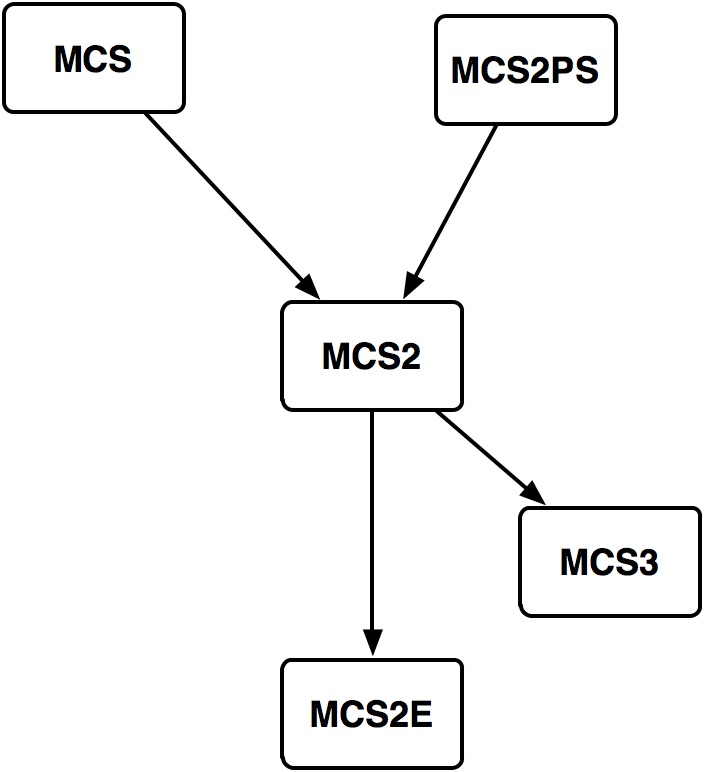
\includegraphics[width=4in]{./mcss/media/mcs-reductions.jpg}

\end{teachnote}

\begin{flex}
\begin{definition}[Subsequence]
\label{def:mcss::introduction::subseq}

A~\defn{subsequence}~$b$ of a sequence~$a$ is a sequence that can be
derived from~$a$ by deleting zero or more elements of~$a$ without changing the
order of remaining elements. 
%
\end{definition}

\begin{example}
\begin{itemize}

\item
The sequence $\cseq{0,2,4}$ is a subsequence of
$\cseq{0,1,2,2,3,4,5}$.

\item
The sequence $\cseq{2,4,3}$ is a not
subsequence of $\cseq{0,1,2,2,3,4,5}$ but $\cseq{2,3,4}$ is.
\end{itemize}
%
\end{example}
\end{flex}

\begin{flex}
\begin{definition}[Contiguous Subsequence]
\label{def:mcss::introduction::consubseq}
A~\defn{contiguous subsequence} is a subsequence that appears
contiguously in the original sequence.
%
For any sequence~$a$ of~$n$ elements, the subsequence
%
\[
b =  a\cirange{i}{j}, 0 \le i \le j < n,
\]
%
consisting of the elements of~$a$ at positions~$i, i+1, \ldots, j$ is
a contiguous subsequence of~$b$.
\end{definition}
%

\begin{example}
For $a = \langle 1, -2, 0, 3, -1, 0, 2, -3 \cseqee$, here are some
contiguous subsequences:
\begin{itemize}
\item 
$\cseqbb 1 \cseqee$,

\item
$\cseqbb -2, 0, 3 \cseqee$, and

\item
$\cseqbb 3, -1,  0, 2, -3 \cseqee$.

\end{itemize}

The sequence~$\cseqbb -1,2,-3 \cseqee$ is not a contiguous subsequence,
even though it is a subsequence.

\end{example}
\end{flex}

\begin{flex}

\begin{definition}[The Maximum Contiguous Subsequence (\MCS{}) Problem]
\label{def:mcss::introduction::mcs-problem}

Given a sequence of integers, 
%
the~\defn{Maximum Contiguous Subsequence Problem} (\MCS{}) requires finding the contiguous subsequence of the sequence with maximum total sum, i.e.,
%
\begin{eqnarray*}
    \MCS{}\,(a) = \argmax{0 \leq i,j < |a|}{\left( \sum_{k=i}^j a[k]  \right)}.
\end{eqnarray*}
%
We define the sum of an empty sequence to be~$\ninfty{}$.
%
\end{definition}

\begin{example}
For 
%
$a = \cseq{1, -2, 0, 3, -1, 0, 2, -3 \cseqee},$ 
%
a maximum contiguous subsequence is, 
%
$\cseq{3, -1, 0, 2}$;
%
another is 
%
$\cseqbb 0, 3, -1, 0, 2 \cseqee.$
%
\end{example}
\end{flex}

%
\begin{flex}
\begin{definition}[The Maximum Contiguous Subsequence Sum (\MCSS{}) Problem]
\label{def:mcss::introduction::mcss-problem}
Given a sequence of integers,
%
the~\defn{Maximum Contiguous Subsequence Sum Problem} (\MCSS{})

%
requires finding
the total sum of the elements in the contiguous subsequence of the
sequence with maximum total sum, i.e.,
%
  \begin{eqnarray*}
    \MCSS{}\,(a) = \max \left\{ \sum_{k=i}^j a[k] \;:\; 0 \leq i,j <
      |a| \right\}.
  \end{eqnarray*}
%
\end{definition}

\begin{example}
For $a = \cseq{1, -2, 0, 3, -1, 0, 2, -3 \cseqee},$ a maximum contiguous
subsequence is, $\cseq{3, -1, 0, 2};$ 
%
another is $\cseqbb 0, 3, -1, 0, 2 \cseqee.$
%
Thus $\MCSS{}~(a) = 4$.

For the empty sequence,~$\MCSS{} = -\infty$ because the sum of an
empty sequence is defined as~$-\infty$.
\end{example}
\end{flex}

\begin{teachnote}
We define $\ninfty{}$ for the empty case instead of $0$ to allow for
negative numbers to matter.
\end{teachnote}

%
\begin{note}
Here we only consider sequences of integers and the addition operation
to compute the sum, the techniques that we describe should apply to
sequences of other types and other associative sum operations.
\end{note}


\begin{gram}[Lower Bound]
To solve the \MCSS{} problem, we need to inspect, at the very least, each and  every element of the sequence.  This requires linear work in the length of the sequence and thus   solve the \MCSS{} problem requires $\Omega(n)$  work.
\end{gram}


\begin{note}[History of the Problem]
\label{not:mcss::introduction::mcss-history}

The study of  maximum contiguous subsequence problem goes to 1970's.  
%
The problem was first proposed in by Ulf Grenander, a Swedish
statistician and a professor of applied mathematics at Brown
University, in 1977.
%
The problem has several names, such maximum subarray sum problem, or
maximum segment sum problem, the former of which appears to be the
name originally used by Grenander.
%
Grenander intended it to be a simplified model for maximum likelihood
estimation of patterns in digitized images, whose structure he wanted
to understand.
%


According to Jon Bentley
%
(Jon Bentley, Programming Pearls (1st edition), page 76.)
%
in 1977, Grenander described the problem to Michael Shamos of
Carnegie Mellon University who overnight designed a divide and
conquer algorithm, which corresponds to our 
%
\href{alg:mcss::dc::first}{first divide-and-conquer algorithm}.
%
When Shamos and Bentley discussed the problem and Shamos' solution,
they thought that it was probably the best possible.
%
A few days later Shamos described the problem and its history at a
Carnegie Mellon seminar attended by statistician Joseph (Jay) Kadane,
who designed the work efficient algorithm within a minute.
%
Kadane's algorithm correspond to the 
%
\href{alg:mcs::iterative}{linear work and span algorithm} 
%
described below.
%



\end{note}


\begin{gram}[Roadmap]
\label{gr:mcss::problem::roadmap}
The remaining sections apply various algorithm-design
techniques to the MCS and \MCSS{} problems.
%
To exercise our vocabulary for algorithm design, the content is
organized to identify carefully the design techniques, sometimes at a
level of precision that may, especially in subsequent reads, feel
pedantic.
%
\end{gram}

%% TODO: ANALYSIS NEED UPDATE.

\section{Brute Force}
\label{sec:mcss::bf}

\begin{gram}
This section presents a first solution to the \MCSS{} problem by using
the \href{sec:design::bf}{brute force technique}.
\end{gram}

\begin{algorithm}[\MCSS{}: Brutest Force]
\label{alg:mcss::bf-alg::brutest}

We can solve the \MCSS{} problem by brute force.
%
First, we identify the set of candidate solutions as the set of all
integers.
%
Then we enumerate all integers and, for each one, check that there is
a contiguous subsequence whose sum is equal to that integer.
%
We stop when we find the largest integer with a matching subsequence.
%


Perhaps obviously, such an algorithm would not terminate, because we
don't know when to stop.
%
Notice, however, that the solution is bounded by the sum of all
positive integers in the sequence.
%
We can thus stop the search when we reach that bound.
%

This algorithm terminates but has the undesirable characteristic that
its bound depends on the values of the elements in the sequence rather
that its length.
\end{algorithm}

\begin{gram}[Reduction to \MCS{}]
\href{alg:mcss::bf-alg::brutest}{Our first algorithm} is rather
inefficient in the worst case, because it tries a large number of
candidate solutions.
%
We can achieve a better bound by reducing \MCSS{} problem to the
\href{def:mcss::introduction::mcss-problem}{Maximum Contiguous Subsequence (\MCS{}) problem}, which requires finding the contiguous subsequence with the
largest sum.
%

The reduction itself is straightforward: because both problems operate
on the same input, there is no need to transform the input.
%
To compute the output, we sum the elements in the sequence returned by
the \MCS{} problem.
%
Using $\cdvar{reduce}$, this requires $O(n)$ work and $O(\lg{n})$ span.
%
Thus, the work and span of the reduction is $O(n)$ and $O(\lg{n})$
respectively.
\end{gram}

\begin{algorithm}[\MCS{}: Brute Force]
\label{alg:mcss::bf-alg::mcs}
We can solve the \MCS{} problem by brute force: we enumerate all
candidate solutions, which consist of all the contiguous subsequences
of the sequence, and find the one with the largest sum.
%
To generate all contiguous subsequences, we can generate all pairs of
integers $(i,j)$, $0 \le i \le j < n$, compute the sum of the
subsequence that corresponds to the pair, and pick the  one with the
largest total.  We write the algorithm as follows:
%
\[
\begin{array}{l}
\cdvar{MCSBF}~a =
\\
~~~~\cd{let} 
\\
~~~~~~~~\cdvar{maxSum}~((i, j, s), (k, \ell, t)) = \cd{if}~s > t~\cd{then}~(i, j, s)~\cd{else}~(k, \ell, t) 
\\
~~~~~~~~b = \cseqbb (i, j, \cdvar{reduce}~+~0~a\cirange{i}{j})  : 0  \le i \le j < n \cseqee
\\
~~~~~~~~(i, j, s) = \cdvar{reduce}~\cdvar{maxSum}~(-1, -1, \ninfty{})~b
\\
~~~~\cd{in}
\\
~~~~~~~~(i, j)
\\
~~~~\cd{end}
\end{array}
\]

\end{algorithm}

\begin{gram}[Cost of Brute Force \MCSS{}]
Using array sequence costs, generating the $n^2$ subsequences requires
a total of $O(n^2)$ work and $O(\lg{n})$ span.
%
Reducing over each subsequence using $\cdvar{reduce}$ adds linear work
per subsequence, bringing the total work to $O(n^3)$. 
%
The final reduce that select the maximal subsequence require $O(n^2)$
work.
%
The total work is thus dominated by the computation of sums for each
subsequence, and therefore is $O(n^3)$.

Because we can generate all pairs in parallel and compute their sum in
parallel in $\Theta(n)$ span using $\cdvar{reduce}$, the algorithm
requires $\Theta(\lg{n})$ span.
\end{gram}


\begin{algorithm}[MCSS: Brute Force]
\label{alg:mcss::bf-alg::mcss}

Our first algorithm uses brute force technique and a reduction to the
\MCS{} problem, which we again solve by brute force using the
\href{alg:mcss::bf-alg::mcs}{brute-force \MCS{} algorithm}.
%
We can write the algorithm as follows:

\[
\begin{array}{l}
\cdvar{MCSSBF}~a =
\\
~~~~\cd{let} 
\\
~~~~~~~~(i, j) =  \cdvar{MCSBF}~a
\\
~~~~~~~~\cdvar{sum} = \cdvar{reduce}~\cstr{+}~0~a\cirange{i}{j}
\\
~~~~\cd{in}
\\
~~~~~~~~\cdvar{sum}
\\
~~~~\cd{end}.
\end{array}
\]
\end{algorithm}


\begin{gram}[Strengthening]
The \href{alg:mcss::bf-alg::mcss}{brute force algorithm} 
%
has some redundancy: to find the solution, it computes the result for
the \MCS{} problem and then computes the sum of the result sequence,
which is already computed by the \MCS{} algorithm.
%
We can eliminate this redundancy by strengthening the \MCS{} problem
and requiring it to return the sum in addition to the subsequence.
%
\end{gram}

\begin{exercise}
Describe the changes to the algorithms 
%
\algref{mcss::bf-alg::mcs} and 
\algref{mcss::bf-alg::mcss}
%
to implement the strengthening described above.
%
How does strengthening impact the work and span costs?
\end{exercise}


\begin{algorithm}[MCSS: Brute Force Strengthened]
\label{alg:mcss::bf-alg::mcss-strong}

We can write the algorithm based on strengthening directly as follows.
%
Because the problem description requires returning only the sum, we
simplify the algorithm by not tracking the subsequences.
%
\[
\begin{array}{l}
\cdvar{MCSSBF}~a =
\\
~~~~\cd{let} 
\\
~~~~~~~~b = \cseqbb \cdvar{reduce}~+~0~a\cirange{i}{j}  : 0  \le i \le j < n \cseqee
\\
~~~~\cd{in}
\\
~~~~~~~~\cdvar{reduce}~\cdvar{max}~\ninfty{}~b
\\
~~~~\cd{end}
\end{array}
\]
\end{algorithm}
%

\begin{flex}
\begin{gram}[Cost Analysis]
%
Let's analyze the work and span of 
%
\href{alg:mcss::bf-alg::mcss-strong}{the strengthened brute-force algorithm} by using 
%
\href{sec:sequences::cost::arrays}{array sequences}
%
and by appealing to our cost bounds for
$\cdvar{reduce}$, $\cdvar{subseq}$, and $\cdvar{tabulate}$.
%
The cost bounds for enumerating all possible subsequences and
computing their sums is as follows.
%
\[
\begin{array}{lllll}
  W(n) & = & 1 + \displaystyle\sum_{1 \leq i\leq j\leq n} W_{\cdvar{reduce}}(j-i) \leq
           1 + n^2 \cdot W_{\cdvar{reduce}}(n) 
       & = & \Theta(n^3) 
\\
  S(n) & = & 1 + \displaystyle\max_{1 \leq i\leq j\leq n} S_{\textrm{reduce}}(j-i) \leq 
           1 + S_{\cdvar{reduce}}(n) 
       & = & \Theta(\lg n) 
\end{array}
\]
%
The final step of the brute-force algorithm is to find the maximum
over these $\Theta(n^2)$ combinations.
%
Since the reduce for this step has $\Theta(n^2)$ work and $\Theta(\lg n)$
span
%
 the cost of the final step is subsumed by other costs analyzed
above.  
%
Overall, we have an $\Theta(n^3)$-work $\Theta(\lg n)$-span algorithm.
\end{gram}

\begin{note}
Note that the span requires the maximum over
%
$\binom{n}{2} \leq n^2$ values, 
%
but since $\lg n^k = k \lg n$, this is simply
%
$\Theta(\lg n)$.
\end{note}
\end{flex}



\begin{gram}[Summary]
  When trying to apply the brute-force technique to the \MCSS{} problem,
  we encountered a problem.  We solved this problem by reducing \MCSS{}
  problem to another problem, \MCS{}. We then realized a redundancy in
  the resulting algorithm and eliminated that redundancy by
  strengthening \MCS{}.  This is a quite common route when designing a
  good algorithm: we find ourselves refining the problem and the
  solution until it is (close to) perfect.
\end{gram}

\section{Applying Reduction}
\label{sec:mcss::reduction}

\begin{gram}
\href{sec:mcss::bf}{In the previous section}, we used the brute-force
technique to develop an algorithm that has logarithmic span but large
(cubic) work.
%
In this section, we apply the reduction technique to obtain a
low span and work-efficient (linear work) algorithm for the \MCSS{}
problem.
\end{gram}

\subsection{Auxiliary Problems}

\begin{gram}[Overlapping Subsequences and Redundancy]
To understand how we might improve the amount of work, observe that
the brute-force algorithm performs a lot of repeated and thus redundant work.
%
To see why, consider the subsequences that start at some location.
For each position, e.g., the middle, the algorithm considers a
subsequence that starts at the position and at any other position that
comes after it.
%
Even though each subsequence differs from another by a single element
(in the ending positions), the algorithm computes the total sum for
each of these subsequences independently, requiring linear work per
subsequence.
%
The algorithm does not take advantage of the overlap between the many subsequences it considers.
\end{gram}

\begin{gram}[Reducing Redundancy]
We can reduce redundancy by taking advantage of the overlaps and
computing all subsequences that start or end at a given position
together.
%
Our basic strategy in applying the reduction technique is to use this
observation.
%
To this end, we define two problems that are closely related to the
\MCSS{} problem, present efficient and parallel algorithm for these
problems, and then reduce the \MCSS{} to them.
\end{gram}


\begin{definition}[\MCSSS{}]
The~\defn{Maximum Contiguous Subsequence Sum with Start},
abbreviated~\defn{\MCSSS{}}, problem requires finding the maximum
contiguous subsequence of a sequence that starts at a given position.
\end{definition}




\begin{definition}[\MCSSE{} Problem]
The~\defn{Maximum Contiguous Subsequence with Ending}, i.e.,
the~\defn{\MCSSE{}} problem requires finding the maximum contiguous
subsequence ending at a specified end position.
\end{definition}


\begin{gram}[Reductions from \MCSS{} to \MCSSS{} and \MCSSE{}]
Observe that we can reduce the \MCSS{} problem to \MCSSS{} problem by
enumerating over all starting positions, solving \MCSSS{} for each
position, and taking the maximum over the results.
%
A similar reduction works for the \MCSSE{} problem.

Because the inputs to all these problems are essentially the same, we
don't need to transform the input.  To compute the output for \MCSS{},
we need to perform a $\cdvar{reduce}$.
%
The reduction itself it thus efficient.
\end{gram}



\begin{algorithm}[\MCSSS{}]
\label{alg:mcss::reduction::mcsss}
We can solve the \MCSSS{} problem by first computing the sum for all
subsequences that start at the given position scan and then finding
their maximum.
%
We can compute the sum for all subsequences starting at a position
efficiently by using a $\cdvar{scan}$.
%
\[
\begin{array}{l}
\cdvar{MCSSSBF}~a~i =
\\ 
~~~~\cd{let} 
\\ 
~~~~~~~~b = \cdvar{scanInc}~\cstr{+}~0~a~\cirange{i}{(|a|-1)}
\\ 
~~~~\cd{in}
\\ 
~~~~~~~~\cdvar{reduce}~\cdvar{max}~\ninfty{}~b
\\ 
~~~~\cd{end}
\end{array}
\]

Because the algorithm performs one scan and one reduce, it performs
(wost-case for any start position) $\Theta(n)$ work in
$\Theta(\lg{n})$ span.

\end{algorithm}
%

\begin{flex}
\begin{algorithm}[\MCSSE{} via Scan]
\label{alg:mcss::reduction:mcsse}
The algorithm below uses scan based on the
intuition described above. 
%
\[
\begin{array}{l}
\cdvar{ScanMCSSE}~a~j=
\\
~~~~\cd{let}
\\
~~~~~~~~(b,v) = \cdvar{scan}~\cstr{+}~0~a\cirange{0}{j}
\\
~~~~~~~~w= \cdvar{reduce}~\cdvar{min}~\infty~b
\\
~~~~\cd{in}
\\
~~~~~~~~v - w 
\\
~~~~\cd{end}
\end{array}
\]


Using array sequences, this algorithm has $\Theta(n)$ work and
$\Theta(\lg n)$ span.
\end{algorithm}
%

\begin{gram}[Intuition for \MCSSE{}]
\label{gr:mcss::reduction::mcsse:simple::intuition}

Any contiguous subsequence of a given sequence can be expressed in
terms of the difference between two prefixes of the sequence:
%
the subsequence $A\cirange{i}{j}$ is equivalent to the difference
between the subsequence $A\cirange{0}{j}$ and the subsequence
$A\cirange{0}{i-1}$.
%

Thus, we can compute the sum of the elements in
a contiguous subsequence as
\[
\cdvar{reduce}~\cstr{+}~0~a\cirange{i}{j}
= 
\left(\cdvar{reduce}~\cstr{+}~0~a\cirange{0}{j}\right)
- 
\left(\cdvar{reduce}~\cstr{+}~0~a\cirange{0}{i-1}\right)
\]
where the ``-'' is the subtraction operation on integers.

This observation leads us to a solution to the \MCSSE{} problem.
%
Consider an ending position $j$ and suppose that we have
the sum for each prefix that ends at $i < j$.
%
Since we can express any subsequence ending at position $j$ by
subtracting the corresponding prefix, we can compute the sum for the
subsequence $A\cirange{i}{j}$ by subtracting the sum for the prefix
ending at $j$ from the prefix ending at $i-1$.
%
Thus the maximum contiguous sequence ending at position $j$ starts at
position $i$ which has the minimum of all prefixes up to $i$.
%
%% \begin{teachnote}
%% Important: We don't need to include $j$ because this would
%%  result in an empty subsequence. We can handle that separately
%%  at the top level.
%% \end{teachnote}
%
We can compute the minimum prefix that comes before $j$ by using just
another scan.  
%
%Furthermore, we can compute the minimum preceeding prefix for all
%positions in a single scan.
%
\end{gram}
\end{flex}
%


\subsection{Reduction to \MCSSS{}}


\begin{teachask}
Can you improve the brute-force algorithm by reducing the \MCSS{}
problem to \MCSSS{} problem?
\end{teachask}
%

\begin{algorithm}[\MCSS{}: Reduced Force]
\label{alg:mcss::reduction::mcss-red-mcsss}

We can find a more efficient brute-force algorithm for \MCSS{} by
reducing the problem to \MCSSS{} and
using \href{alg:mcss::reduction::mcsss}{the algorithm for it}.

The idea is to try all possible start positions, solve the \MCSSS{}
problem for each, and select their maximum.
%
The code for the algorithm is shown below.
%
\[
\begin{array}{l}
\cdvar{RBFMCSS}~a = 
\\
~~~~\cdvar{reduce}~\cdvar{max}~\ninfty{}~\cseq{(\cdvar{BFMCSSS})~a~i : 0 \le i < n}.
\end{array}
\]
In the worst case, the algorithm performs $\Theta(n^2)$ work in
$\Theta(\lg{n})$ span, delivering a linear-factor improvement in
work.
\end{algorithm}
%

\begin{remark}
\algref{mcss::reduction::mcsss} is an optimal algorithm for \MCSSS{}
because it requires $O(n-i)$ work for starting position~$i$.
%
By reducing \MCSS{} to \MCSSS{}, we were able to eliminate certain
kinds of redundancy (those that occur when computing the maximum for
subsequences that start at a given position) but not all.
%
In the next section, we will see, how to improve our bound further.
\end{remark}

\subsection{Reduction to \MCSSE{}}

\begin{algorithm}[MCSS by Reduction to \MCSSE{}]
\label{alg:mcss::reduction:mcss-red-mcsse}

We can solve the \MCSS{} problem by enumerating all instances of
the \MCSSE{} problem and selecting the maximum.
%
\[
\begin{array}{l}
\cdvar{ScanMCSS}~a=
\\
~~~~\cdvar{reduce}~\cdvar{max}~\ninfty~\cseq{(\cdvar{ScanMCSSE}~a~i) : 0 \le i < |a|}
\end{array}
\]

This algorithm has $O(n^2)$ work and $O(\lg{n})$ span.

\end{algorithm}

\begin{proposition}[Overlaps and \MCSSE{}]
\label{prop:mcss::reduction::mcsse-overlaps}
Suppose that we are given the maximum contiguous sequence, $M_{i}$
ending at position~$i$.
%
We can compute the maximum contiguous sequence ending at position~$i+1$,
$M_{i+1}$, from this by noticing that 
%
\begin{itemize}
\item $M_{i+1} = \kwappend{M_{i}}{\cseq{a[i]}},$ or 
\item $M_{i+1} = \cseq{a[i]},$
\end{itemize}
%
depending on the sum for each.
\end{proposition}

\begin{exercise}
Prove that 
%
\href{prop:mcss::reduction::mcsse-overlaps}{the proposition above}
%
is correct.
\end{exercise}


%% \begin{teachnote}
%% Why is this correct?  There cannot be a smaller subsequence contained
%% in the left one because if so, the returned sequence would not be maximum.
%% \end{teachnote}


\begin{gram}
The algorithm for solving \MCSS{} by reduction to \MCSSE{} solves many
instances of \MCSSE{} in parallel.
%
If we give up some parallelism, it turns out that we can improve the
work efficiency further based on
\propref{mcss::reduction::mcsse-overlaps}.
%
The idea is to iterate over the sequence and solve the \MCSSE{}
problem for each ending position.
%
To solve the \MCSSE{} problem, we then take the maximum over all
positions.
%
\end{gram}

\begin{algorithm}[\MCSS{} with Iteration]
\label{alg:mcs::iterative}
The \PML code for the algorithm for \MCSS{} obtained by reduction to
\MCSSE{} is shown below.
%
% in \algref{mcs::iterative}.
%
We use the function $\cdvar{iteratePrefixes}$ to iterate over the input
sequence and construct a sequence whose $i^{th}$ position contains the
solution to the \MCSSE{} problem at that position.

\[
\begin{array}{l}
\cdvar{IterativeMCSS}~a = 
\\
~~~~\cd{let}
\\ 
~~~~~~~~f~(\cdvar{sum},x) =
\\
~~~~~~~~~~~~\cd{if}~\cdvar{sum} + x \ge x~\cd{then}
\\ 
~~~~~~~~~~~~~~~~\cdvar{sum} + x
\\
~~~~~~~~~~~~\cd{else}
\\
~~~~~~~~~~~~~~~~x
\\ 
~~~~~~~~b = \cdvar{iteratePrefixes}~f~\ninfty{}~a
\\
~~~~\cd{in}
\\
~~~~~~~~\cdvar{reduce}~\cdvar{max}~\ninfty{}~b
\\
~~~~\cd{end}
\end{array}
\] 
\end{algorithm}

\begin{gram}[Cost Analysis]
Let's analyze the work and span of this algorithm.
%
We first have to decide the cost specification of sequences that we
want to use.
%
The algorithm only uses $\cdvar{iteratePrefixes}$ and $\cdvar{reduce},$ we
can therefore use array sequences.
%
Note now that the function $f$ performs constant work in constant
span, we thus have $W(n) = O(n)$ and $S(n) = O(n)$.
%
\end{gram}





\begin{gram}
\href{alg:mcs::iterative}{Using reduction and iteration}, we designed an algorithm that is work efficient, which performs asymptotically optimal work.
%
But unfortunately the algorithm is completely sequential.
%
We now present a work-efficient and low-span algorithm
for the \MCSS{} problem by reducing it to \MCSSE{} and using the
$\cdvar{scan}$ to solve the resulting \MCSSE{} instances.
\end{gram}

\begin{gram}[Intuition behind the Algorithm]
\label{gr:mcss::reduction:mcsse::optimal-reduction::intution}



We presented an
\href{gr:mcss::reduction::mcsse:simple::intuition}{observation} for solving the \MCSSE{} problem: the maximal contiguous
subsequence ending at a given position can be found by subtracting the
sum for the prefix at that position from the minimum sum over all
preceeding prefixes.

For our new algorithm, we use the same intuition but refine it
further by noticing that
\begin{itemize}
\item we can compute the sum for all prefixes in the sequence in one
  scan, and
\item we can compute the minimum prefix sum preceeding all positions
  in the sequence in one scan.
\end{itemize}

After computing these quantities, all that remains is to take the
difference and select the maximum.
%
\end{gram}


\begin{flex}
\begin{algorithm}[MCSS: Work Optimal and Low Span]
The algorithm below shows a scan-based algorithm based on the
\href{gr:mcss::reduction:mcsse::optimal-reduction::intution}{intuition described above.}
%
\[
\begin{array}{l}
\cdvar{ScanMCSS}~a =
\\
~~~~\cd{let}
\\
~~~~~~~~(b,v) = \cdvar{scan}~\cstr{+}~0~a
\\
~~~~~~~~c = \cdvar{append}~b~\cseq{v}
\\
~~~~~~~~(d,\_) = \cdvar{scan}~\cdvar{min}~\infty~c
\\
~~~~~~~~e = \cseq{c[i]-d[i]: 0 < i < |a|}
\\
~~~~\cd{in}
\\
~~~~~~~~\cdvar{reduce}~\cdvar{max}~\ninfty{}~e
\\
~~~~\cd{end}
\end{array}
\]
\end{algorithm}
%


\begin{example}
\label{ex:mcs:scan-based}
Consider the sequence $a$
\[
a = \cseq{1, -2, 0, 3, -1, 0, 2, -3}.
\]

Compute
\[
\begin{array}{lcl}
(b,v) & = & \cdvar{scan}~\cdvar{+}~0~a
\\
c  & = & \cdvar{append}~ b~ \cseq{v}.
\end{array}
\]
We have $c =  \cseq{0, 1, -1, -1, 2, 1, 1, 3, 0}$.

The sequence~$c$ contains the prefix sums ending at each position,
including the element at the position; it also contains the empty
prefix.

% \begin{teachnote}
%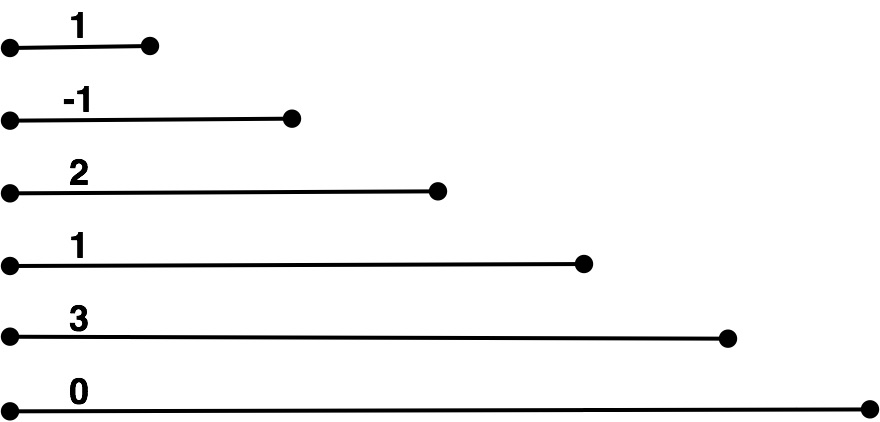
\includegraphics[width=3in]{maximum-contiguous-subsequence/mcss-scan-generic}
%\end{teachnote}

Using the sequence $c$, we can find the minimum prefix up to all
positions as
\[
(d,\_) = \cdvar{scan}~\cdvar{min}~\infty~c
\]
to obtain
\[
d = \cseq{\infty, 0, 0, -1, -1 -1, -1, -1, -1}.
\]

We can now find the maximum subsequence ending at any position $i$ by
subtracting the value for $i$ in $c$ from the value for all the prior
prefixes calculated in $d$.
%

Compute
\[
\begin{array}{lcl}
e & = & \cseq{c[i]-d[i]: 0 < i < |a|} 
\\
  & = & \cseq{1, -1, 0, 3, 2, 2, 4, 1}.
\end{array}
\]

It is not difficult to verify in this small example that the values in
$e$ are indeed the maximum contiguous subsequences ending in each
position of the original sequence.  Finally, we take the maximum of
all the values is $e$ to compute the result
\[
\cdvar{reduce}~\cdvar{max}~\ninfty{}~e = 4.
\]

\end{example}
\end{flex}

\begin{gram}[Cost of the Algorithm]

Using array sequences, and the fact that addition and minimum take
constant work, the algorithm performs $\Theta(n)$ work in $\Theta(\lg
n)$ span.  
%
The algorithm is work optimal because any algorithm must inspect each
and every element of the sequence to solve the \MCSS{} problem.
\end{gram}

\section{Divide And Conquer}
\label{sec:mcss::dc}

\subsection{A First Solution}
\label{sec:mcss::dc::first}

\begin{flex}
\begin{gram}[Diving the Input]
To apply divide and conquer, we first need to figure out how to divide the input.
%
There are many possibilities, but dividing the input in two halves is
usually a good starting point, because it reduces the input for both
subproblems equally, reducing thus the size of the largest component,
which is important in bounding the overall span.
%
Correctness is usually independent of the particular strategy of
division.
%

Let us divide the sequence into two halves, recursively solve the
problem on both parts, and combine the solutions to solve the original
problem.
\end{gram}

\begin{example}
\label{ex:mcss1}
Let $a = \cseq{1, -2, 0, 3, -1, 0, 2, -3}$.  By using the approach, we
divide the sequence into two sequences $b$ and $c$ as follows
\[
b = \cseq{1, -2, 0, 3}
\]
and
\[
c = \cseq{-1, 0, 2, -3}
\]
%
We can now solve each part to obtain $3$ and $2$ as the solutions to
the subproblems.
%
Note that there are multiple sequences that yield the maximum sum.  
\end{example}
\end{flex}

\begin{teachask}
How can we combine the solutions for the two halves to solve the
original problem?
\end{teachask}
%

\begin{gram}[Using Solutions to Subproblems]
To construct a solution for the original problem from those of the
subproblems, let's consider where the solution subsequence might come
from.  There are three possibilities.
\begin{enumerate}
\item  
The maximum sum lies completely in the left subproblem.

\item 
The maximum sum lies completely in the right subproblem.

\item
The maximum sum overlaps with both halves, spanning the cut.
\end{enumerate}

The three cases are illustrated below

\begin{center}
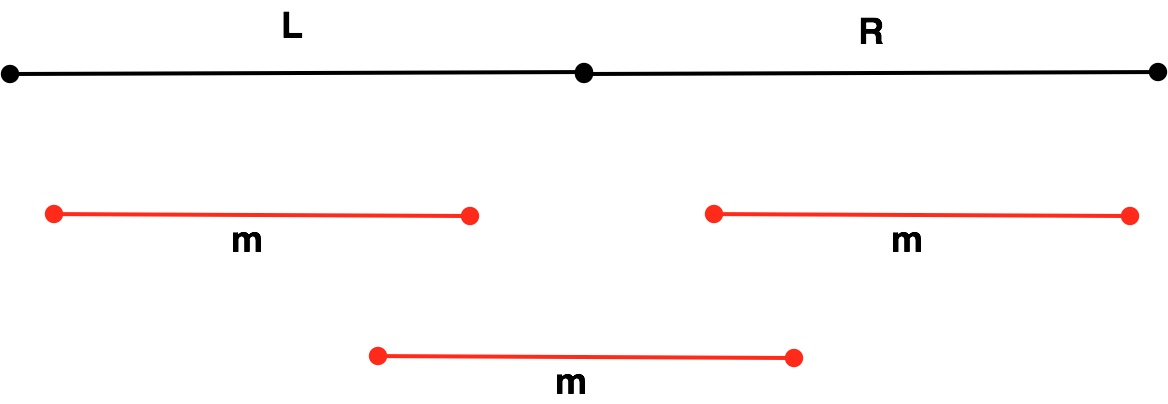
\includegraphics[width=4.5in]{./mcss/media/mcss-dandc-simple.jpg}
\end{center}

The first two cases are already solved by the recursive calls, but not
the last.  Assuming we can find the largest subsequence that spans the
cut, we can write our algorithm as shown below.
\end{gram}


\begin{algorithm}[Simple Divide-and-Conquer for MCSS]
\label{alg:mcss::dc::first}
Using a function called $\cdvar{bestAcross}$ to find the largest
subsequence that spans the cut, we can write our algorithm as follows.

\[
\begin{array}{l}
\cdvar{MCSSDC}~a =
\\
~~~~\cd{if}~ |a| = 0~\cd{then}
\\
~~~~~~~~\ninfty{}
\\
~~~~\cd{else if}~|a| = 1 ~\cd{then}
\\ 
~~~~~~~~a[0]
\\
~~~~\cd{else}
\\ 
~~~~~~~~\cd{let}
\\ 
~~~~~~~~~~~~(b, c)  = \cdvar{splitMid}~a
\\ 
~~~~~~~~~~~~(m_b, m_c) = \left( \cdvar{MCSSDC}~b \ ||\ \cdvar{MCSSDC}~c \right)
\\ 
~~~~~~~~~~~~m_{bc} = \cdvar{bestAcross}~(b, c)
\\ 
~~~~~~~~\cd{in}
\\ 
~~~~~~~~~~~~\max\{m_b, m_c, m_{bc}\}
\\ 
~~~~~~~~\cd{end}
\end{array} 
\]
\end{algorithm}

%% \begin{question}
%%   Can you find an algorithm for finding the subsequence with the
%%   largest sum that spans the cut (i.e.,
%%   \texttt{bestAcross}$(L,R)$)?  Hint: try the problem-reduction
%%   technique to reduce the problem to another one that we know.
%% \end{question}

\begin{flex}
\begin{algorithm}[Maximum Subsequence Spanning the Cut]
\label{alg:mcss::dc::first::bestacross}

We can reduce the problem of finding the maximum subsequence spanning
the cut to two problems that we have seen already:
Maximum-Contiguous-Subsequence Sum with Start, \MCSSS{}, and
Maximum-Contiguous-Subsequence Sum at Ending, \MCSSE{}.
%
The maximum sum spanning the cut is the sum of the largest suffix on
the left plus the largest prefix on the right.  
%
The prefix of the right part is easy as it directly maps to the
solution of \MCSSS{} problem at position $0$.
%
Similarly, the suffix for the left part is exactly an instance of
\MCSSE{} problem.
%
We can thus use the algorithms that we have seen in the previous
section for solving this problem,
\algref{mcss::reduction::mcsss},
%
and, 
%
\algref{mcss::reduction:mcsse}
respectively.

The cost of both of these algorithms is $\Theta(n)$ work and
$\Theta(\lg{n})$ span and thus the total cost is also the same.
\end{algorithm}

\begin{example}
%In \exref{mcss1}
In the example above, the largest suffix on the left is $3$, which is
given by the sequence 
$\cseq{3}$ or $\cseq{0, 3}$.

%
The largest prefix on the right is $1$ given by the sequence
$\cseq{-1, 0, 2}$.
%
Therefore the largest sum that crosses the middle is $3 + 1 = 4$.
\end{example}
\end{flex}

\subsubsection{Correctness}
\label{sec:mcss::dc::first::correctness}

\begin{gram}
%
%% \begin{question}
%% What technique can we use to show that our divide-and-conquer
%% algorithm is correct?
%% \end{question}
%
%As described in \chref{divide-and-conquer}, to prove a

To prove a divide-and-conquer algorithm correct, we use the technique
of strong induction, which enables to assume that correctness remains
correct for all smaller subproblems.
%
We now present such a correctness proof for the algorithm~$\cdvar{MCSSDC}$.
\end{gram}

\begin{flex}
\begin{theorem}[Correctness of the algorithm $\cdvar{MCSSDC}$]
  Let $a$ be a sequence. The algorithm $\cdvar{MCSSDC}$ returns the
  maximum contiguous subsequence sum in a gives sequence---and returns
  $\ninfty{}$ if $a$ is empty.
\end{theorem}

\begin{proof}
The proof will be by (strong) induction on length of the input
sequence.  Our induction hypothesis is that the theorem above holds
for all inputs smaller than the current input.
%

We have two base cases: one when the sequence is empty and one when it
has one element.  
%
On the empty sequence, the algorithm returns $\ninfty{}$ and thus the
theorem holds.
%
On any singleton sequence $\cseqbb x \cseqee$, the \MCSS{} is $x$,
because
\[
\max \left\{ \sum_{k=i}^j a[k] \;:\; 0 \leq i <
    1, 0 \leq j < 1 \right\} = \sum_{k=0}^0 a[0] = a[0] = x\,.
\]
%
The theorem therefore holds.

For the inductive step, let $a$ be a sequence of length $n \ge 1$, and
assume inductively that for any sequence $a'$ of length $n' < n$, the
algorithm correctly computes the maximum contiguous subsequence sum.
%
Now consider the sequence $a$ and let $b$ and $c$ denote the left and
right subsequences resulted from dividing $a$ into two parts (i.e.,
$\cdvar{(b, c) = splitMid a}$).  
%
Furthermore, let $a\cirange{i}{j}$ be any contiguous subsequence of $a$
that has the largest sum, and this value is $v$.  
%
Note that the proof has to account for the possibility that there may
be many other subsequences with equal sum.  
%
Every contiguous subsequence must start somewhere and end after it.
We consider the following $3$ possibilities corresponding to how the
sequence $a\cirange{i}{j}$ lies with respect to $b$ and $c$:

\begin{itemize}
\item 
If the sequence $a\cirange{i}{j}$ starts in $b$ and ends $c$. Then its
sum equals its part in $b$ (a suffix of $b$) and its part in $c$ (a
prefix of $c$).  
%
If we take the maximum of all suffixes in $c$ and
prefixes in $b$ and add them this is equal the maximum of all
contiguous sequences bridging the two, because $\max\cset{x + y : x
  \in X, y \in Y\}} = \max\cset{x \in X} + \max\cset{y \in Y}$. 
%
By assumption this equals the sum of $a\cirange{i}{j}$ which is $v$.
Furthermore by induction $m_b$ and $m_c$ are sums of other
subsequences so they cannot be any larger than $v$ and hence
$\max\{m_b, m_c, m_{bc}\} = v$.


\item 
If $a\cirange{i}{j}$ lies entirely in $b$, then it follows from our
inductive hypothesis that $m_b = v$.  Furthermore $m_c$ and $m_{bc}$
correspond to the maximum sum of other subsequences, which cannot be
larger than $v$. 
%
So again $\max\{m_b, m_c, m_{bc}\} = v$.

\item Similarly, if $a_{i..j}$ lies entirely in $c$, then it follows
  from our inductive hypothesis that $m_c = \max\{m_b, m_c, m_{bc}\} =
  v$.

\end{itemize}

We conclude that in all cases, we return $\max\{m_b, m_c, m_{bc}\} = v$,
as claimed.
\end{proof}
\end{flex}

\subsubsection{Cost Analysis}
\label{sec:mcss::dc::first::cost}

\begin{gram}
%
%% \begin{todo}
%% We have given a log span algorithm for prefix but not for suffix.  we
%% should to that.
%% \end{todo}
%
By \algref{mcss::dc::first::bestacross}, we know that the maximum
subsequence crossing the cut in $\Theta(n)$ work and $\Theta(\lg{n})$
span.
%
Note also that $\cdvar{splitMid}$ requires  $O(\lg n)$ work and span using
array or tree sequences.
%
% This yields the following recurrences
We thus have the following recurrences with array-sequence or
tree-sequence specifications
%
\begin{align*}
  W(n) &= 2W(n/2) + \Theta(n)\\
  S(n) &= S(n/2) +  \Theta(\lg n).
\end{align*}
%% showt: if O(1) work and span, then span is S(n) &=& S(n/2) + O(1)

Using the definition of big-$\Theta$, we know
that
\begin{align*}
  W(n) &\leq 2W(n/2) + k_1\cdot n + k_2,
\end{align*}
where $k_1$ and $k_2$ are constants.
%
By using the tree method, we can conclude that $W(n) = \Theta(n\lg{n})$ and
$S(n) = \lg^2{n}$.
%

%% We can also arrive at the same answer by mathematical induction.  If
%% you want to go via this route (and you don't know the answer a
%% priori), you'll need to guess the answer first and check it.  This is
%% often called the ``substitution method.''  Since this technique relies
%% on guessing an answer, you can sometimes fool yourself by giving a
%% false proof.  The following are some tips:
%% \begin{enumerate}
%% \item Spell out the constants. Do not use the asymptotic notation---we
%%   need to be precise about constants, the asymptotic notation makes it
%%   super easy to fool ourselves.

%% \item Be careful that the inequalities always go in the right direction.

%% \item Add additional lower-order terms, if necessary, to make the
%%   induction go through.
%% \end{enumerate}
\end{gram}

\begin{gram}[Solving the Recurrence Using Substitution Method]
Let's now redo the recurrences above using the substitution method.
%
Specifically, we'll prove the following theorem using (strong)
induction on $n$.
%
\end{gram}

\begin{flex}
\begin{theorem}
  Let a constant $k > 0$ be given.  If $W(n) \leq 2 W(n/2) + k \cdot n$ for $n >
  1$ and $W(1) \leq k$ for $n \leq 1$, then we can find constants $\kappa_1$ and
  $\kappa_2$ such that \[ W(n) \;\leq\; \kappa_1 \cdot n \lg n + \kappa_2.\]
\end{theorem}

\begin{proof}
  Let $\kappa_1 = 2k$ and $\kappa_2 = k$.  For the base case ($n=1$), we check
  that $W(1) = k \leq \kappa_2$.  For the inductive step ($n>1$), we assume that
  \[
  W(n/2) \leq \kappa_1 \cdot \tfrac{n}2 \lg (\tfrac{n}2) + \kappa_2,
  \]
  And we'll show that $W(n) \leq \kappa_1 \cdot n \lg n + \kappa_2$.  To show
  this, we substitute an upper bound for $W(n/2)$ from our assumption into the
  recurrence, yielding
  \begin{align*}
    W(n) \;&\leq\; 2W(n/2) + k \cdot n  \\
    \;&\leq\; 2(\kappa_1 \cdot \tfrac{n}2 \lg (\tfrac{n}2) + \kappa_2) + k \cdot n\\
    \;&=\; \kappa_1 n (\lg n - 1) + 2 \kappa_2 + k \cdot n\\
    \;&=\; \kappa_1 n \lg n + \kappa_2 + (k \cdot n + \kappa_2 - \kappa_1 \cdot n)\\
    \;&\leq\; \kappa_1 n \lg n + \kappa_2,
  \end{align*}
  where the final step follows because $k \cdot n + \kappa_2 - \kappa_1 \cdot n \leq
  0$ as long as $n > 1$.
\end{proof}
\end{flex}

\begin{teachnote}
Using divide and conquer, we were able to reduce work to
$\Theta(n\lg{n})$ from $\Theta(n^2)$, which was the bound that we
obtained using the brute-fore algorithm.
%
%% \begin{question}
%% Where did the savings come from?
%% \end{question}
%
The improved brute-force algorithm still performs poorly, because it
performs  redundant work by considering seperately subsequences
that overlap significantly.  
%
\end{teachnote}


\subsection{Divide And Conquer with Strengthening}

\begin{gram}
Our first divide-and-conquer algorithm performs $O(n \lg n)$ work,
which is $O(\lg{n})$ factor more than the optimal.
%
In this section, we shall reduce the work to $O(n)$ by being more
careful about avoiding redundant work.
%
%\begin{question}
%Is there some redundancy in our first divide-and-conquer algorithm?
%\end{question}
%
\end{gram}


%\begin{question}
%Can we avoid re-computing the maximum prefix and suffix?
%\end{question}



\begin{gram}[Intuition]
Our divide-and-conquer algorithm has an important redundancy: the
maximum prefix and maximum suffix are computed recursively to solve
the subproblems for the two halves but are computed again at the
combine step of the divide-and-conquer algorithm.
%

Because these are computed as part of solving the subproblems, we
could return them from the recursive calls.  
%
To do this, we will strengthen the problem so that it returns the
maximum prefix and suffix.  
%
This problem, which we shall call~\defn{\MCSSPS{}}, matches the
original \MCSS{} problem in its input and returns strictly more
information.
% 
Solving \MCSS{} using \MCSSPS{} is therefore trivial.  
%
We thus focus on the \MCSSPS{} problem.
\end{gram}

%% \begin{question}
%% Can you see how we can update our divide and conquer algorithm to
%% solve the \MCSSPS{} problem, i.e., to return also the maximum prefix and
%% suffix in addition to maximum contiguous subsequence?
%% \end{question}
%

\begin{gram}[Solving MCSSPS]
We can solve this problem by strengthening our divide-and-conquer
algorithm from the previous section.
%
We need to return a total of three values: 
\begin{itemize}
\item the max subsequence sum,
%
\item the max prefix sum, and
%
\item the max suffix sum.
\end{itemize}
%

At the base cases, when the sequence is empty or consists of a single
element, this is easy to do.
%
For the recursive case, we need to consider how to produce the desired
return values from those of the subproblems.
Suppose that the two subproblems return  $(m_1, p_1, s_1)$ and $(m_2, p_2, s_2)$.
%% \begin{question}
%% How can we compute the result from the solutions to the subproblems? 
%% \end{question}

One possibility to compute as result
\[
  (\max(s_1+p_2, m_1, m_2), p_1, s_2).
\]


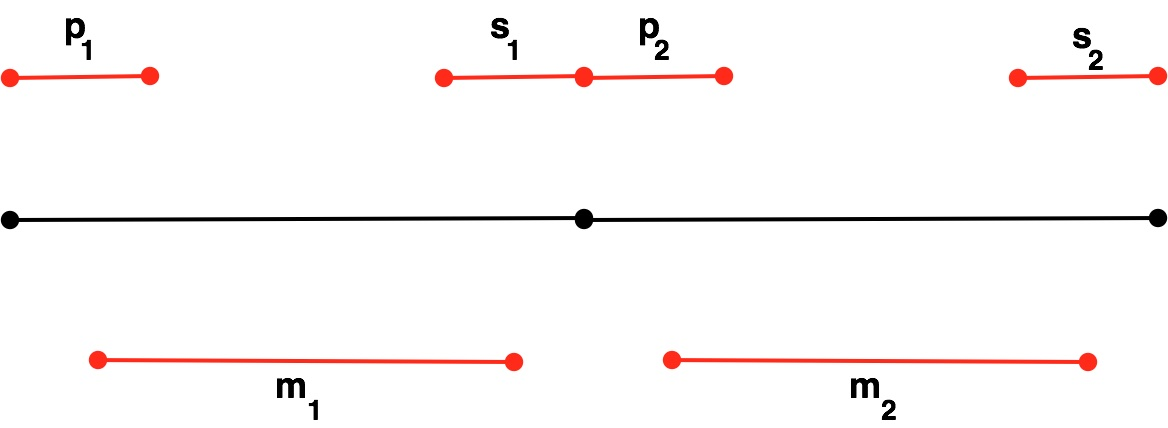
\includegraphics[width=4.5in]{./mcss/media/mcss-dandc.jpg}

%% \begin{question}
%% Don't we have consider the case when $s_1$ or $p_2$ is the maximum? 
%% \end{question}

Note that we don't have to consider the case when $s_1$ or $p_2$ is
the maximum, because that case is checked in the computation of $m_1$
and $m_2$ by the two subproblems.
%
%% \begin{question}
%% Are the prefix and suffix correct?  Can we not have a bigger prefix
%% that contains all of the first sequence?
%% \end{question}


This solution fails to account for the case when the suffix and
prefix can span the whole sequence.
%
%% \begin{todo}
%% Give an example.
%% \end{todo}
%% %
%% \begin{question}
%% How can you fix this problem? 
%% \end{question}
%

We can fix this problem by returning the total for each subsequence so
that we can compute the maximum prefix and suffix correctly.  Thus, we
need to return a total of four values: 
\begin{itemize}
\item the max subsequence sum,
\item the
max prefix sum, 
\item the max suffix sum, and 
\item the overall sum.
\end{itemize}
%

Having this information from the subproblems is enough to produce a
similar answer tuple for all levels up, in constant work and span per
level. Thus what we have discovered is that to solve the strengthened
problem efficiently we have to strengthen the problem once again.
Thus if the recursive calls return $(m_1, p_1, s_1, t_1)$ and $(m_2,
p_2, s_2, t_2)$, then we return
\[
  (\max(s_1+p_2, m_1, m_2), \max(p_1,
  t_1+p_2), \max(s_1+t_2, s_2), t_1+t_2).
\]
%
\end{gram}


%
\begin{algorithm}[Linear Work Divide-and-Conquer MCSS]
\[
\begin{array}{l}
\cdvar{MCSSDCAux}~a = 
\\
~~~~\cd{if}~|a| = 0~\cd{then}
\\
~~~~~~~~(\ninfty{},\ninfty{},\ninfty{},0)
\\
~~~~\cd{else}~if |a| = 1 \cd{then}
\\
~~~~~~~~(a[0], a[0], a[0], a[0])
\\
~~~~\cd{else}
\\
~~~~~~~~\cd{let} 
\\
~~~~~~~~~~~~(b,c) = \cdvar{splitMid}~a 
\\
~~~~~~~~~~~~((m_1, p_1, s_1, t_1), (m_2, p_2, s_2, t_2)) = (\cdvar{MCSSDCAux}~b~\cpar{}~\cdvar{MCSSDCAux}~c)
\\
~~~~~~~~\cd{in} 
\\
~~~~~~~~~~~~(\cdvar{max}~(s_1+p_2, m_1, m_2),   
\\
~~~~~~~~~~~~~\cdvar{max}~(p_1, t_1+p_2),      
\\
~~~~~~~~~~~~~\cdvar{max}~(s_1+t_2, s_2),     
\\
~~~~~~~~~~~~~t_1+t_2)              
\\
~~~~~~~~\cd{end}
\\
\cdvar{MCSSDC}~a = 
\\
~~~~\cd{let} 
\\
~~~~~~~~(m, \_, \_, \_) = \cdvar{MCSSDCAux}~a 
\\
~~~~\cd{in}
\\
~~~~~~~~m 
\\
~~~~\cd{end}
\end{array}
\]
\end{algorithm}

%% \cdvar{MCSSDC}~a = 
%% \\
%% ~~~~\cd{let} 
%% \\
%% ~~~~~~~~(m,_,_,_) = \cdvar{MCSSDCAux}~a 
%% \\
%% ~~~~\cd{in}
%% \\
%% ~~~~~~~~m 
%% \\
%% ~~~~\cd{end}


%% \\
%% ~~~~~~~~~~~~(\cdvar{max}~ (s_1+p_2, m_1, m_2),   \cdc{overall mcss}
%% \\
%% ~~~~~~~~~~~~\cdvar{max}~ (p_1,t_1+p_2),      \cdc{maximum prefix}
%% \\
%% ~~~~~~~~~~~~\cdvar{max}~ (s_1+t_2, s_2),     \cdc{maximum suffix}
%% \\
%% ~~~~~~~~~~~~t_1+t_2)              \cdc{total sum}
%% \\
%% ~~~~~~~~\cd{end}
%% \\
%% ~~~~~~~~(m,_,_,_) = \cdvar{MCSSDC'}~a
%% \\
%% ~~~~~~~~\cd{in} 
%% \\
%% ~~~~~~~~~~~~m 
%% \\
%% ~~~~~~~~\cd{end}
%% \\
%% \cdvar{MCSSDC}~a = 
%% \\
%% ~~~~\cd{let} 
%% \\
%% ~~~~~~~~(m,_,_,_) = \cdvar{MCSSDC'}~ a 
%% \\
%% ~~~~\cd{in}
%% \\
%% ~~~~~~~~m 
%% \\
%% ~~~~\cd{end}


\begin{gram}[Cost Analysis]
Since $\cdvar{splitMid}$ requires $O(\lg n)$ work and
span in both array and tree sequences, we have
\begin{align*}
  W(n) &= 2 W(n/2) + O(\lg n)\\
  S(n) &= S(n/2) + O(\lg n).
\end{align*}
%
The $O(\lg{n})$ bound on $\cdvar{splitMid}$ is not tight for array sequences, where $\cdvar{splitMid}$ requires $O(1)$ work, but this loose upper bound suffices to achieve the bound on the work that we seek.
%
Note that the
span is the same as before, so we'll focus on analyzing the work.  Using the
tree method, we have
\begin{center}
  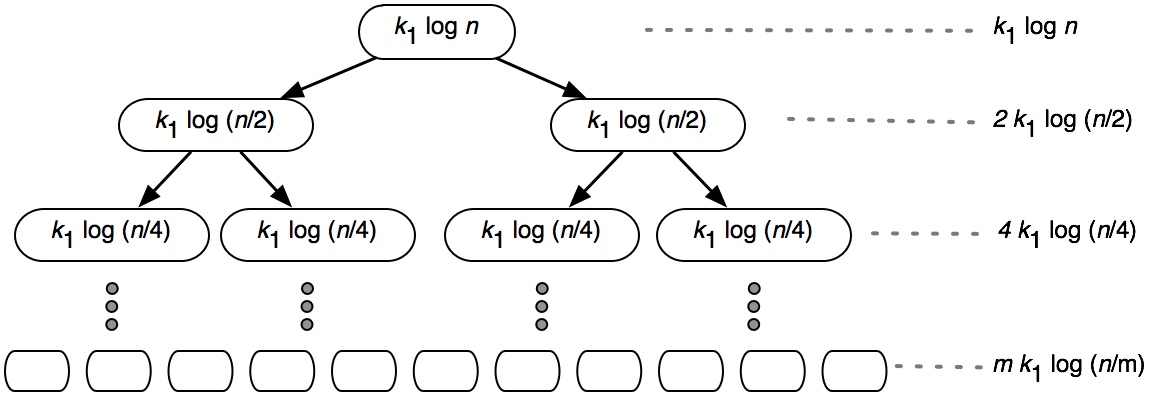
\includegraphics[width=5in]{./mcss/media/recurtree2.jpg}
\end{center}

Therefore, the total work is upper-bounded by
\begin{eqnarray*}
  W(n) &\leq& \sum_{i=0}^{\lg n} k_1 2^i \lg (n/2^i)
\end{eqnarray*}

It is not so obvious to what this sum evaluates, but we can bound it
as follows:
\begin{align*}
  W(n) &\leq \sum_{i=0}^{\lg n} k_1 2^i \lg (n/2^i) \\
  &= \sum_{i=0}^{\lg n} k_1 \pparen{2^i\lg n - i\cdot 2^i} \\
  &= k_1\pparen{\sum_{i=0}^{\lg n} 2^i}\lg n - k_1\sum_{i=0}^{\lg n} i\cdot 2^i\\
  &= k_1(2n - 1)\lg n - k_1\sum_{i=0}^{\lg n} i\cdot 2^i.
\end{align*}

We're left with evaluating $s = \sum_{i=0}^{\lg n} i\cdot 2^i$.  Observe that
if we multiply $s$ by $2$, we have
\[
2s = \sum_{i=0}^{\lg n} i\cdot 2^{i+1} = \sum_{i=1}^{1 + \lg n} (i-1)2^i,
\]
so then
\begin{align*}
s &= 2s - s \;=\; \sum_{i=1}^{1 + \lg n} (i-1)2^i - \sum_{i=0}^{\lg n} i\cdot 2^i\\
&= \pparen{(1 + \lg n)  - 1}2^{1 + \lg n} - \sum_{i=1}^{\lg n} 2^i \\
&= 2n\lg n - (2n -2).
\end{align*}
Substituting this back into the expression we derived earlier, we have $W(n)
\leq k_1(2n - 1)\lg n - 2k_1(n \lg n - n + 1) \in O(n)$ because the $n\lg n$
terms cancel.
\end{gram}

\begin{gram}
We can solve the recurrency by using substitution method also.  We'll
make a guess that $W(n) \leq \kappa_1 n - \kappa_2 \lg n - k_3$.
More precisely, we prove the following theorem.
\end{gram}

\begin{flex}
\begin{theorem}
  Let $k > 0$ be given.  If $W(n) \leq 2 W(n/2) + k \cdot \lg n$ for $n > 1$
  and $W(n) \leq k$ for $n \leq 1$, then we can find constants $\kappa_1$,
  $\kappa_2$, and $\kappa_3$ such that \[ W(n) \;\leq\; \kappa_1 \cdot n -
  \kappa_2 \cdot \lg n - \kappa_3.\]
\end{theorem}

\begin{proof}
  Let $\kappa_1 = 3k$, $\kappa_2 = k$, $\kappa_3 = 2k$. We begin with
  the base case. Clearly, $W(1) = k \leq \kappa_1 - \kappa_3 = 3k - 2k = k$.
  For the inductive step, we substitute the inductive hypothesis into
  the recurrence and obtain
  \begin{align*}
    W(n) &\leq 2W(n/2) + k \cdot \lg n\\
    &\leq 2 (\kappa_1 \tfrac{n}2 - \kappa_2 \lg (n/2) - \kappa_3) + k \cdot\lg n\\
    &= \kappa_1 n - 2 \kappa_2 (\lg n - 1) - 2 \kappa_3 + k \cdot \lg n\\
    &= (\kappa_1 n - \kappa_2 \lg n - \kappa_3) +
    (k \lg n - \kappa_2 \lg n + 2 \kappa_2 - \kappa_3) \\
    &\leq \kappa_1 n - \kappa_2 \lg n - \kappa_3,
  \end{align*}
  where the final step uses the fact that $(k \lg n - \kappa_2 \lg n +
  2 \kappa_2 - \kappa_3) = (k \lg n - k \lg n + 2 k - 2 k) = 0 
 \leq 0$ by our choice of $\kappa$'s.
\end{proof}
\end{flex}




